\begingroup
\emergencystretch=1em
\section{Experiment P2D: reliability at a fixed attempted exchange budget}
\label{sec:p2d}
\subsection{Question and frozen comparison}
P2C found that cyclic rotation was already competitive with specialized selection on the four-node Gaussian benchmark. P2D asks how that conclusion changes when attempted ranges fail to arrive or arrive with misleading values. It separates missing information from corrupted information and evaluates a fixed innovation gate as a distinct estimator comparison.

The four paths, \SI{60}{s} duration, \SI{100}{Hz} IMU, \SI{10}{Hz} opportunity grid, initialization, noise levels, EKF process model, and 20 seeds remain those of P2A--P2C. Every run spends exactly \textbf{360 attempted undirected exchanges}, or 10\% of the P2A full-rate count. Cyclic and information selection share the per-tick allocation in Eq.~\ref{eq:p2c_capacity}, with one pair at each of 360 active ticks. The information score remains the predicted centered-position covariance reduction from P2C. The P2B \SI{1}{Hz} all-six-link schedule is rerun under each stress. Its count is equal but its timing differs, so it is a contextual reference rather than an isolated test of pair choice.

For each seed, potential Gaussian ranges, reception outcomes, and outlier values are generated for \emph{all six pairs at all time indices} before scheduling. IMU and initial-velocity draws are identical to P2A--P2C. Reception and outlier fields use separate random streams; 30\% and 50\% loss threshold the same uniform reception field. The latter therefore contains every potential failure in the former, although adaptive schedules can choose different pairs. Policies selecting the same pair at the same time see identical potential measurements and failures. Their realized successful counts need not be equal.

Selection occurs after inertial prediction and \emph{before} revealing current reception or range quality. A failed or rejected exchange consumes its attempt; there are no retries, replacements, known bad-link labels, or oracle availability information. Information selection reacts through the covariance resulting from previous accepted updates. Cyclic and uniform schedules remain fixed.

\subsection{Reliability cases and fixed gate}
The seven cases in Table~\ref{tab:p2d_protocol} are separate stresses rather than mixtures. Interval endpoints follow \([t_0,t_1)\): a range at the ending time is available again. Implementation node indices start at zero, corresponding to node 1 and link 1--2 in this report.
\begin{table}[htbp]
\centering
\caption{Predefined P2D stresses. Received ranges retain Gaussian noise with \(\sigma_r=\SI{0.12}{m}\).}
\label{tab:p2d_protocol}
\begin{tabular}{lp{9.8cm}}
\toprule
Case & Modification to potential measurements \\
\midrule
Clean & All ranges received, Gaussian noise only. \\
30\% / 50\% loss & Independent Bernoulli loss across pairs and time, probability 0.30 or 0.50. \\
Network outage & All links unavailable from 20 to \SI{30}{s}. \\
Node 1 outage & Its three incident links unavailable from 20 to \SI{30}{s}; the other three remain available. \\
Positive outliers & Independently, 5\% of potential ranges gain a positive bias uniform from 1 to \SI{3}{m}. \\
Persistent link bias & Link 1--2 gains \SI{0.75}{m} from 20 to \SI{40}{s}; other links remain Gaussian. \\
\bottomrule
\end{tabular}
\end{table}

The ordinary (naive) EKF is run for all seven cases and three schedules. The gated EKF is run for clean, network-outage, outlier, and persistent-bias cases: \(20\times3\times(7+4)=660\) runs. The gate is fixed before evaluation:
\begin{equation}
 \mathrm{NIS}_{ij,k}=\frac{(z_{ij,k}-\hat r_{ij,k})^2}{H_{ij,k}P_kH_{ij,k}^{\top}+\sigma_r^2},
 \qquad\text{accept if }\mathrm{NIS}_{ij,k}\leq9.
\end{equation}
For simultaneous ranges, each gate uses the current state and covariance after earlier accepted ranges in the fixed pair order. Rejection leaves both unchanged. This nominal three-standard-deviation innovation test is not an NLOS classifier or a demonstrated consistency guarantee for the nonlinear EKF. Its threshold is not fitted to the results. The gate receives no corruption labels; the selector does not discount a pair after rejection.

Three counts remain distinct: \(C_{\rm attempt}=360\), \(C_{\rm received}\leq C_{\rm attempt}\), and \(C_{\rm accepted}\leq C_{\rm received}\). Received minus accepted counts rejections. Attempted exchanges define communication cost, including failures and rejected measurements. This is a count proxy; airtime, retries, and radio energy are not simulated.

Whole-run fleet, worst-node, centroid, relative-shape, yaw, and windowed shape RMSE use native \SI{100}{Hz} histories. Compact curves are sampled at \SI{2}{Hz}. Mean and sample standard deviation describe the 20 seeds. Clean ordinary-EKF endpoints reproduce all committed P2B/P2C values in every seed to numerical tolerance. Paired differences use 30,000 paired-seed bootstrap resamples with descriptive percentile 95\% intervals. These intervals are not corrected for multiple comparisons and cover stochastic realizations of fixed paths.

\subsection{Ordinary EKF: missing versus misleading ranges}
Table~\ref{tab:p2d_naive} gives the complete ordinary-EKF comparison. Shape removes the instantaneous mean position error, as in P2A--P2C; it does not rotate estimates to align with truth.
\begin{table}[htbp]
\centering\small
\caption{P2D naive EKF, 20 seeds and 360 attempted exchanges per run. Received and accepted counts are means; fleet and worst-node RMSE are means in metres; shape RMSE is mean \(\pm\) sample standard deviation in metres.}
\label{tab:p2d_naive}
\begin{tabular}{llrrrrr}
\toprule
Stress & Schedule & Received & Accepted & Fleet & Worst & Shape \\
\midrule
Clean & Cyclic & 360.0 & 360.0 & 1.061 & 1.086 & \(0.0824\pm0.0159\) \\
 & Information & 360.0 & 360.0 & 1.060 & 1.083 & \(0.0789\pm0.0141\) \\
 & All links, 1 Hz & 360.0 & 360.0 & 1.061 & 1.085 & \(0.0858\pm0.0164\) \\
\addlinespace
30\% loss & Cyclic & 251.5 & 251.5 & 1.062 & 1.087 & \(0.0919\pm0.0179\) \\
 & Information & 252.4 & 252.4 & 1.061 & 1.087 & \(0.0939\pm0.0195\) \\
 & All links, 1 Hz & 253.0 & 253.0 & 1.063 & 1.092 & \(0.1002\pm0.0240\) \\
\addlinespace
50\% loss & Cyclic & 175.0 & 175.0 & 1.064 & 1.100 & \(0.1100\pm0.0203\) \\
 & Information & 179.4 & 179.4 & 1.064 & 1.097 & \(0.1065\pm0.0199\) \\
 & All links, 1 Hz & 178.3 & 178.3 & 1.065 & 1.106 & \(0.1164\pm0.0300\) \\
\addlinespace
Network outage & Cyclic & 300.0 & 300.0 & 1.061 & 1.089 & \(0.0917\pm0.0158\) \\
 & Information & 300.0 & 300.0 & 1.062 & 1.088 & \(0.0898\pm0.0132\) \\
 & All links, 1 Hz & 300.0 & 300.0 & 1.062 & 1.090 & \(0.0993\pm0.0211\) \\
\addlinespace
Node 1 outage & Cyclic & 330.0 & 330.0 & 1.062 & 1.090 & \(0.0883\pm0.0156\) \\
 & Information & 305.1 & 305.1 & 1.061 & 1.085 & \(0.0853\pm0.0131\) \\
 & All links, 1 Hz & 330.0 & 330.0 & 1.062 & 1.087 & \(0.0892\pm0.0151\) \\
\addlinespace
Positive outliers & Cyclic & 360.0 & 360.0 & 1.102 & 1.191 & \(0.2955\pm0.0664\) \\
 & Information & 360.0 & 360.0 & 1.106 & 1.193 & \(0.3024\pm0.0558\) \\
 & All links, 1 Hz & 360.0 & 360.0 & 1.100 & 1.190 & \(0.2830\pm0.0505\) \\
\addlinespace
Persistent bias & Cyclic & 360.0 & 360.0 & 1.073 & 1.148 & \(0.1690\pm0.0119\) \\
 & Information & 360.0 & 360.0 & 1.069 & 1.122 & \(0.1478\pm0.0127\) \\
 & All links, 1 Hz & 360.0 & 360.0 & 1.074 & 1.149 & \(0.1718\pm0.0133\) \\
\addlinespace
\bottomrule
\end{tabular}
\end{table}

For cyclic, 30\% and 50\% independent loss reduce mean received counts to 251.5 and 175.0 and raise mean shape RMSE from \SI{0.0824}{m} to \SI{0.0919}{m} and \SI{0.1100}{m}. Fleet RMSE changes only from about \SI{1.061}{m} to \SI{1.064}{m}. A ten-second network outage receives 300 ranges and gives \SI{0.0917}{m} shape RMSE. Substantial missing data degrades relative accuracy but does not cause catastrophic failure for these paths and duration.

Five percent positive outliers instead increase cyclic shape RMSE to \SI{0.2955}{m}, despite accepting all 360 ranges; the persistent biased link gives \SI{0.1690}{m}. About 16.6 received cyclic outliers per seed cause much more damage than 50\% packet loss. Received count alone therefore does not describe useful information.
\begin{figure}[htbp]
\centering
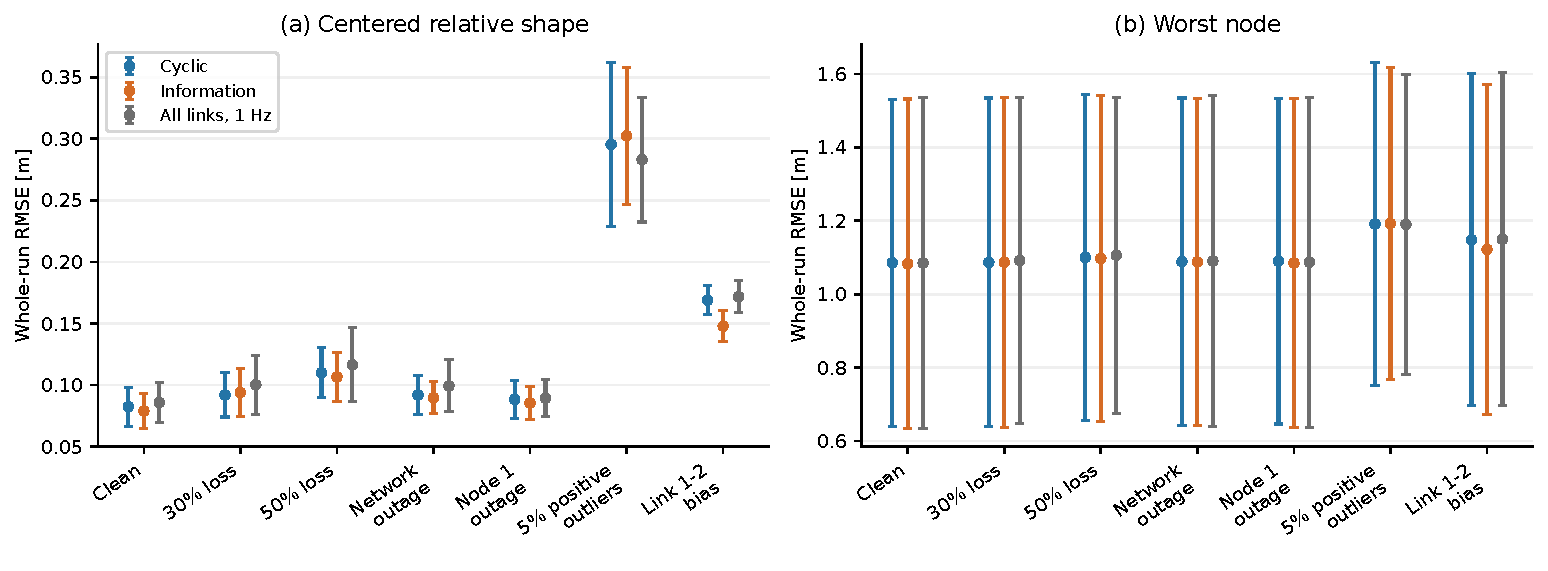
\includegraphics[width=\textwidth]{figures/phase2/p2d_reliability.pdf}
\caption{Ordinary-EKF relative-shape and worst-node RMSE at 360 attempts. Markers show across-seed means; bars show one sample standard deviation, not confidence intervals. Uniform all-link timing differs from the matched cyclic/information timing.}
\label{fig:p2d_reliability}
\end{figure}

Information does not establish a general advantage over cyclic under missing data. Mean paired shape differences are \(+0.00206\)~m at 30\% loss, \(-0.00344\)~m at 50\% loss, \(-0.00198\)~m under network outage, and \(-0.00296\)~m under node outage; every bootstrap interval spans zero. Its ordinary outlier difference is \(+0.00699\)~m, interval \([-0.02933,0.04339]\)~m.

Persistent bias is an exception: ordinary information improves on ordinary cyclic by \(-0.02117\)~m, interval \([-0.02632,-0.01577]\)~m, with 18/20 wins. It selects the biased link only 12.9 times on average during the bias interval, versus cyclic's 20. This is a consequence of covariance-driven choices under this specific bias and geometry, not evidence that it identifies NLOS.

\subsection{Outage recovery and failed-link selection}
After network reception resumes at \SI{30}{s}, ordinary cyclic shape RMSE over \([30,40)\)~s is \SI{0.0927}{m}, versus clean \SI{0.0732}{m}. Over \([40,60]\)~s it is \SI{0.0629}{m}, close to clean \SI{0.0627}{m}. Information gives \SI{0.0845}{m} and \SI{0.0636}{m}, versus clean \SI{0.0664}{m} and \SI{0.0633}{m}. Fixed-window summaries show recovery toward clean accuracy; they do not estimate a universal recovery time. The stored 30--40 s metric is a post-outage window, but remains inside the active bias interval in the persistent-bias case; post-bias recovery is evaluated over 40--60 s.

The node outage exposes a communication-efficiency issue. Cyclic loses exactly 30 attempts and receives 330 ranges. Information loses 54.9 attempts on average and receives only 305.1. About 91.5\% of its 60 choices during the outage are incident to the unavailable node. Uncertainty not reduced by successful updates continues to attract its information score. It has no availability model or explicit response to failed reception. Similar shape accuracy despite fewer successful ranges does not make those attempts free or establish that this behavior is desirable.

\subsection{Gating: outlier protection and persistent-bias interaction}
\begin{table}[htbp]
\centering\small
\caption{P2D gated EKF, 20 seeds and 360 attempted exchanges per run. Received and accepted counts are means; fleet and worst-node RMSE are means in metres; shape RMSE is mean \(\pm\) sample standard deviation in metres.}
\label{tab:p2d_gated}
\begin{tabular}{llrrrrr}
\toprule
Stress & Schedule & Received & Accepted & Fleet & Worst & Shape \\
\midrule
Clean & Cyclic & 360.0 & 359.2 & 1.061 & 1.085 & \(0.0824\pm0.0157\) \\
 & Information & 360.0 & 359.1 & 1.060 & 1.081 & \(0.0810\pm0.0164\) \\
 & All links, 1 Hz & 360.0 & 359.0 & 1.061 & 1.085 & \(0.0870\pm0.0160\) \\
\addlinespace
Network outage & Cyclic & 300.0 & 299.3 & 1.061 & 1.089 & \(0.0918\pm0.0155\) \\
 & Information & 300.0 & 299.3 & 1.062 & 1.086 & \(0.0913\pm0.0158\) \\
 & All links, 1 Hz & 300.0 & 299.5 & 1.062 & 1.091 & \(0.1002\pm0.0212\) \\
\addlinespace
Positive outliers & Cyclic & 360.0 & 342.8 & 1.061 & 1.086 & \(0.0838\pm0.0164\) \\
 & Information & 360.0 & 340.9 & 1.059 & 1.085 & \(0.0826\pm0.0147\) \\
 & All links, 1 Hz & 360.0 & 342.2 & 1.061 & 1.086 & \(0.0888\pm0.0157\) \\
\addlinespace
Persistent bias & Cyclic & 360.0 & 337.9 & 1.067 & 1.094 & \(0.0956\pm0.0624\) \\
 & Information & 360.0 & 293.9 & 1.069 & 1.122 & \(0.1305\pm0.0444\) \\
 & All links, 1 Hz & 360.0 & 338.9 & 1.063 & 1.100 & \(0.0993\pm0.0288\) \\
\addlinespace
\bottomrule
\end{tabular}
\end{table}

Gating reduces positive-outlier cyclic shape RMSE from \SI{0.2955}{m} to \SI{0.0838}{m}, about 71.6\%, close to clean accuracy, accepting 342.8 ranges on average. Information falls from \SI{0.3024}{m} to \SI{0.0826}{m}, accepting 340.9. All schedules improve in all 20 seeds; cyclic's gate-minus-ordinary difference is \(-0.21166\)~m, interval \([-0.24196,-0.18303]\)~m. Clean gated runs reject approximately one range per seed and have broadly similar accuracy to ordinary clean runs. Network-outage gated results also remain close to ordinary results. For these isolated large errors, rejection has a much larger effect than specialized pair selection.
\begin{figure}[htbp]
\centering
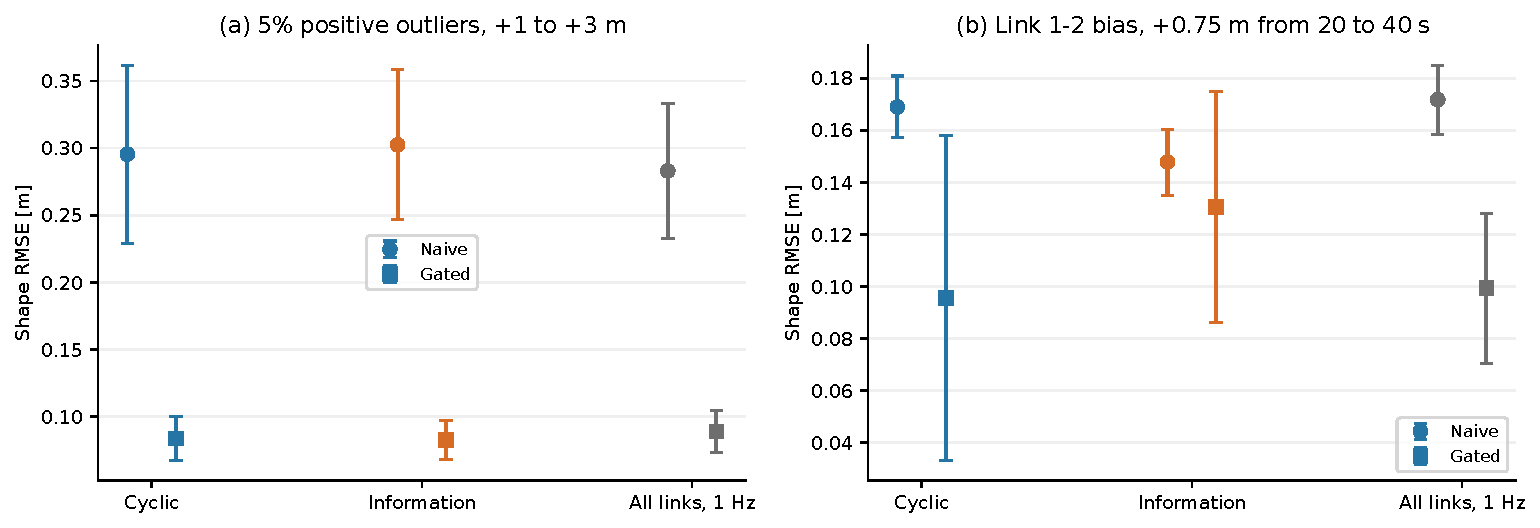
\includegraphics[width=\textwidth]{figures/phase2/p2d_gating.pdf}
\caption{Ordinary and gated shape RMSE under positive outliers and persistent bias. Bars show one across-seed sample standard deviation. The fixed gate strongly protects against isolated errors, while persistent bias exposes an interaction with information selection.}
\label{fig:p2d_gate}
\end{figure}

Under persistent bias, gated cyclic improves from \SI{0.1690}{m} to \SI{0.0956}{m}, accepting 337.9 ranges and improving 19/20 seeds. Its \SI{0.0624}{m} sample standard deviation indicates uneven protection. Gated information reaches \SI{0.1305}{m}, accepting only 293.9 ranges. Its improvement over ordinary information is \(-0.01730\)~m, interval \([-0.03376,0.00270]\)~m, spanning zero. It is worse than gated cyclic by \(+0.03484\)~m, interval \([0.01997,0.04804]\)~m, winning only 1/20 seeds. Gating thus reverses the ordinary policy ranking for this case.

During the bias interval, gated information selects the biased link 59.7 times on average, about 49.8\% of 120 attempts. Cyclic selects it 20 times (16.7\%); ordinary information selects it 12.9 times (10.8\%). Rejection preserves covariance uncertainty and the unchanged score continues favoring the link. This is consistent with repeated unproductive selection and fewer updates on other links. The logs establish attempt concentration and its coincident accuracy cost; P2D does not test a reliability-aware replacement or isolate every causal error mechanism.

After bias ends at \SI{40}{s}, gated cyclic shape RMSE over \([40,60]\)~s is \SI{0.0810}{m}, whereas gated information remains at \SI{0.1489}{m}; clean gated values are \SI{0.0631}{m} and \SI{0.0646}{m}. Rejecting a persistent bias does not automatically guarantee prompt recovery or good use of the remaining budget.
\begin{figure}[htbp]
\centering
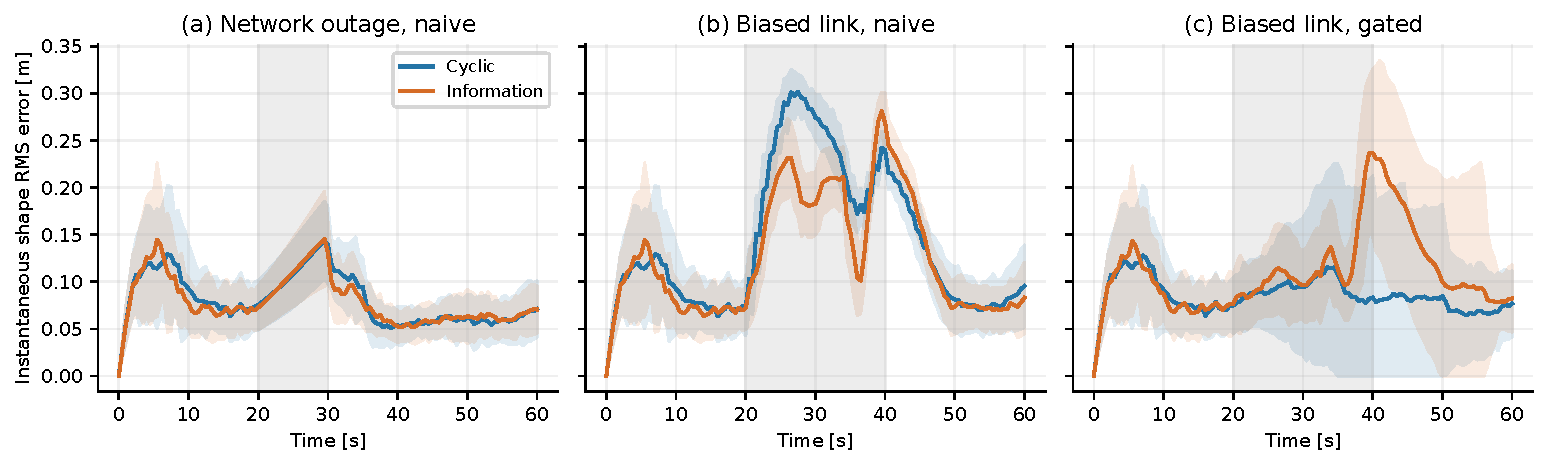
\includegraphics[width=\textwidth]{figures/phase2/p2d_time_profiles.pdf}
\caption{Instantaneous shape RMS error: pointwise mean \(\pm\) one sample standard deviation over 20 seeds, clipped at zero. Grey shading marks network outage (20--30 s) or link bias (20--40 s). Bands show seed variability, not confidence intervals for the mean.}
\label{fig:p2d_time}
\end{figure}
\begin{figure}[htbp]
\centering
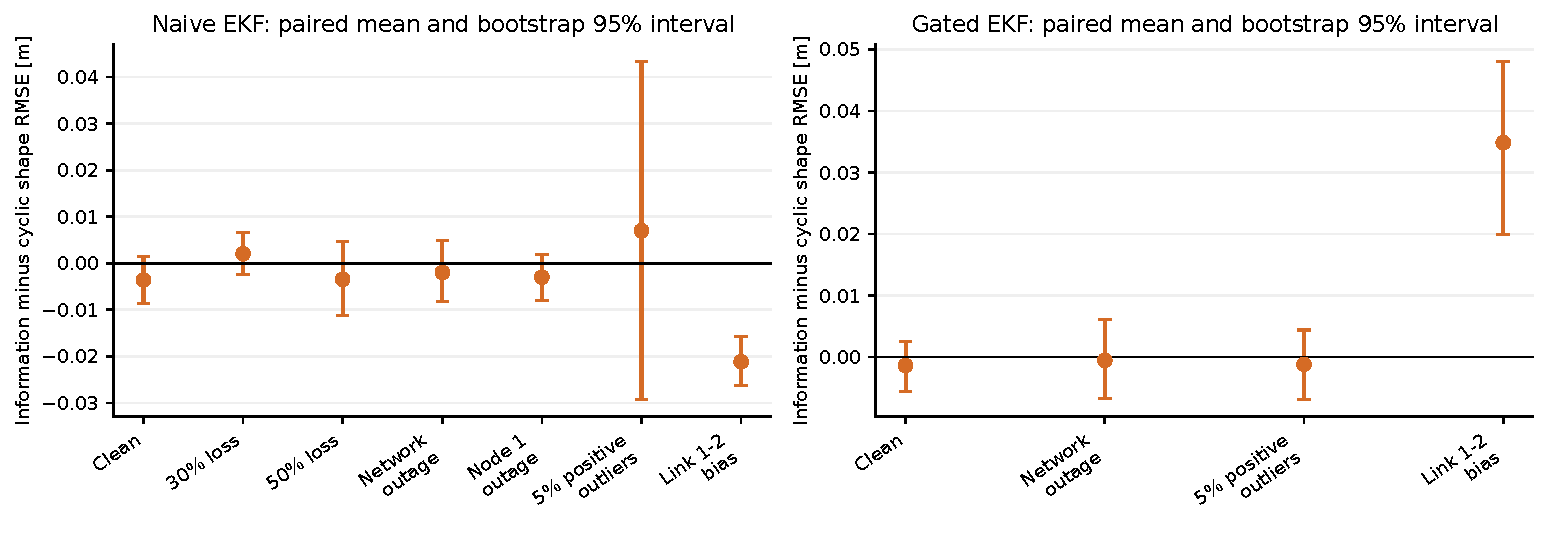
\includegraphics[width=\textwidth]{figures/phase2/p2d_paired_differences.pdf}
\caption{Information-minus-cyclic whole-run shape RMSE. Markers show paired means; bars show descriptive paired-seed bootstrap percentile 95\% intervals, without multiple-comparison correction. Negative values favor information. The gated panel includes only the four predefined gate cases.}
\label{fig:p2d_paired}
\end{figure}

\subsection{Decision, limits, and P2E handoff}
Retain cyclic as the practical reference. Under missing data, information's advantage is small or uncertain and it can repeatedly attempt unavailable links. Under isolated large positive errors, the gate provides a clear and much larger benefit. Under persistent bias, the gate and unchanged information score can concentrate attempts on a rejected link and worsen recovery. Received and accepted counts must accompany the attempted budget.

The benchmark remains infrastructure-free: centroid RMSE near \SI{1.056}{m} in clean conditions dominates fleet RMSE, and pairwise ranges cannot correct the unobservable common translation. P2D covers one budget, fixed paths, seven stylized stresses, and a fixed gate. Failure distributions and timing are not calibrated to hardware. It does not validate energy, retries, NLOS classification, gate tuning, estimator consistency, combined failures, or learned link reliability.

Proceed to \textbf{P2E: IMU sensitivity} using cyclic as the primary schedule and retaining explicit ordinary/gated comparisons where corruption is studied. A future reliability-aware score should combine predicted information with evidence of reception or acceptance and be tested against gated cyclic at equal attempts. That is a separate experiment; P2D does not justify silently replacing the score or tuning the gate on this campaign.
\endgroup
